%! Unidad 12 — Energía y trabajo: la energía y sus propiedades, trabajo mecánico, energía cinética (teorema de las fuerzas
%! vivas), fuerzas conservativas y energía potencial (gravitatoria y elástica), conservación de la energía mecánica, fuerzas no
%! conservativas, potencia y rendimiento (teoría, ejemplos resueltos, ejercicios por apartados, lectura, prácticas y situación de
%! aprendizaje)
%! Fuente: Fuentes/Fisica/Unidad 12 (capturas 439 —portada, mitad derecha— y 440-451, solucionario) y Unidad 13 (captura 452:
%!   «Experimenta en casa» y autoevaluación de este tema).
%! Texto reescrito; datos de los ejercicios cambiados (y más realistas cuando los de la fuente no lo eran) y recalculados; g = 9,8 m/s².
%! Figuras en images/UD12/: nuevas en html/ (caminos_peso, rendimiento, montana_looping, practica_carrete) y copiadas (PDF + SVG)
%!   de 4ESO/images/UD11 (trabajo_casos, trabajo_angulo, energia_cinetica, energia_potencial, muelle, conservacion,
%!   rozamiento_energia). Gráficas con pgfplots (trabajo como área, energía potencial elástica, energías en una caída).

\section*{Para empezar: una máquina que devora roca}
\addcontentsline{toc}{section}{Para empezar: una máquina que devora roca}

Para abrir los túneles del metro o del AVE se usan \textbf{tuneladoras}: enormes cilindros de acero, de hasta \qty{15}{\m} de
diámetro, cuya cabeza giratoria tritura la roca mientras la máquina avanza y coloca a su paso los anillos de hormigón del túnel. En
un día pueden excavar decenas de metros, un trabajo que a mano costaría meses. ¿De dónde sale la energía que necesitan? ¿Cuánta se
aprovecha de verdad para excavar y cuánta se pierde? ¿Cómo podrían ser más eficientes?

Casi todo lo que nos rodea funciona gracias a algún tipo de \textbf{energía} y supone realizar algún \textbf{trabajo}. En el lenguaje
de cada día usamos estas palabras con mucha libertad; en esta unidad les daremos un significado preciso y estudiaremos dos ideas muy
potentes: el \textbf{teorema de las fuerzas vivas} y la \textbf{conservación de la energía mecánica}, que permiten resolver muchos
problemas sin necesidad de conocer la aceleración en cada instante. Terminaremos con la \textbf{potencia} y el \textbf{rendimiento},
que miden lo rápido y lo bien que una máquina hace su trabajo.

%========================================================================================
\section{Recuerda de la ESO}\label{sec:ud12-eso}
%========================================================================================

\paragraph{La energía.} Es la causa de todos los cambios que observamos: para mover un objeto, cambiar su posición, deformarlo,
calentarlo o quemarlo interviene la energía. Nuestro organismo la obtiene al metabolizar los nutrientes de los alimentos.

\paragraph{Formas de energía.} \textbf{Mecánica} (asociada al movimiento y a la posición), \textbf{eléctrica} (asociada a la corriente
eléctrica), \textbf{nuclear} (almacenada en los núcleos atómicos), \textbf{química} (almacenada en los enlaces), \textbf{térmica}
(asociada a la agitación de las partículas; la que pasa de un cuerpo caliente a otro más frío se llama \textbf{calor}) y
\textbf{radiante} o electromagnética (la que transportan la luz, las microondas o los rayos X).

\paragraph{Fuentes de energía.} Son los recursos de los que se obtiene energía. Las \textbf{no renovables} (carbón, petróleo, gas
natural, uranio) existen en cantidad limitada y acabarán por agotarse; las \textbf{renovables} (sol, viento, agua, biomasa, calor
interno de la Tierra) son inagotables o se regeneran deprisa. Para alcanzar los Objetivos de Desarrollo Sostenible hay que usar cada
vez más las renovables, que contaminan menos y reducen la dependencia energética de los países.

\begin{exercise}
    Clasifica estas fuentes de energía en renovables y no renovables: carbón, viento, uranio, restos de poda, gas natural, calor del
    interior de la Tierra, radiación solar, mareas.
    \begin{solu}
        \textcolor{red}{Renovables}: viento, restos de poda (biomasa), calor interno de la Tierra (geotérmica), radiación solar y mareas.
        \textcolor{red}{No renovables}: carbón, uranio y gas natural.
    \end{solu}
\end{exercise}

%========================================================================================
\section{La energía: historia del concepto y propiedades}\label{sec:ud12-energia}
%========================================================================================

Hasta ahora hemos estudiado el movimiento a partir de las fuerzas. En muchas situaciones resulta más cómodo cambiar de enfoque y
relacionar las fuerzas con los \textbf{cambios} que producen en un sistema. Para ello necesitamos uno de los conceptos más abstractos
de la física.

\begin{definition}[Energía]
    Es la capacidad que tienen los sistemas físicos para producir cambios en el estado de reposo o de movimiento de otros sistemas con
    los que interaccionan, o en ellos mismos.
\end{definition}

La idea se fue construyendo poco a poco. A finales del siglo \textsc{xvii}, mientras Newton establecía las leyes del movimiento,
\textbf{Gottfried Leibniz} buscaba qué magnitud se conserva en los choques y propuso la \textit{vis viva} («fuerza viva»),
\(m\,v^2\), antecedente de la energía cinética. La palabra \textit{energía} viene del griego \textit{enérgeia}, «actividad»; a principios
del siglo \textsc{xix}, \textbf{Thomas Young} la empleó para la capacidad de un cuerpo para realizar trabajo. Hacia 1842, \textbf{Julius
Robert von Mayer}, médico alemán, y poco después \textbf{James Prescott Joule}, con sus medidas del equivalente mecánico del calor,
establecieron el \textbf{principio de conservación de la energía}. En honor a Joule, la unidad de energía del SI es el \textbf{julio}
(J).

\begin{definition}[Propiedades de la energía]
    \textbf{1. Se conserva}: la energía total de un sistema aislado (y del universo) permanece constante; no se crea ni se destruye.

    \textbf{2. Se transforma}: pasa de unas formas a otras (la química de la gasolina se transforma en cinética del coche).

    \textbf{3. Se transfiere}: pasa de unos cuerpos a otros mediante trabajo, calor u ondas.

    \textbf{4. Se degrada}: en cada transformación, parte de ella acaba como energía térmica a baja temperatura, menos útil.

    \textbf{5. Se almacena y se transporta}: en baterías, embalses o combustibles, y por tendidos eléctricos o gasoductos.
\end{definition}

Según el tipo de interacción o la forma en que se almacena, distinguimos estas formas de energía (tabla~\ref{tab:ud12-formas}):

\begin{table}[H]
    \centering
    \caption{Formas de energía}
    \vspace{-5pt}
    \begin{tabular}{@{}lL{10.5cm}@{}}
        \toprule
        \textbf{Forma} & \textbf{Asociada a\dots} \\
        \midrule
        Mecánica & la posición y el movimiento de los cuerpos (cinética y potencial). \\[3pt]
        Térmica & la agitación de las partículas; está relacionada con la temperatura. \\[3pt]
        Química & los enlaces entre átomos; se libera o se absorbe en las reacciones químicas. \\[3pt]
        Nuclear & las fuerzas que mantienen unido el núcleo; se libera en la fisión y en la fusión. \\[3pt]
        Eléctrica & el movimiento de cargas entre puntos con distinto potencial. \\[3pt]
        Electromagnética & las ondas electromagnéticas, como la luz, las microondas o los rayos X. \\
        \bottomrule
    \end{tabular}
    \label{tab:ud12-formas}
\end{table}

\begin{exercise}
    Pon un ejemplo cotidiano de cada una de las cinco propiedades de la energía.
    \begin{solu}
        \textcolor{red}{Respuesta abierta}. Por ejemplo: se conserva (la energía de un péndulo ideal), se transforma (una placa solar
        convierte la radiante en eléctrica), se transfiere (una taza caliente calienta la mano), se degrada (los frenos de una bici se
        calientan), se almacena y se transporta (la batería del móvil; la red eléctrica).
    \end{solu}
\end{exercise}

\begin{exercise}
    ¿Qué forma de energía interviene en cada caso? a) Un arco tensado. b) Las ondas de un horno microondas. c) La fusión en el núcleo
    del Sol. d) La batería de un patinete. e) Se derrite un cubito de hielo. f) El alumbrado de una calle. g) Pagar con el móvil
    acercándolo al datáfono.
    \begin{solu}
        a) \textcolor{red}{Potencial elástica}. b) \textcolor{red}{Electromagnética}. c) \textcolor{red}{Nuclear}. d)
        \textcolor{red}{Química} (que se transforma en eléctrica). e) \textcolor{red}{Térmica} (calor). f) \textcolor{red}{Eléctrica},
        que se transforma en luminosa. g) \textcolor{red}{Electromagnética} (ondas de radio de corto alcance).
    \end{solu}
\end{exercise}

%========================================================================================
\section{El trabajo}\label{sec:ud12-trabajo}
%========================================================================================

En la vida diaria llamamos «trabajo» a cualquier actividad que exija esfuerzo físico o mental. En física, en cambio, el trabajo es
la \textbf{energía que una fuerza transfiere} a un cuerpo al desplazarlo: si no hay desplazamiento, no hay trabajo
(figura~\ref{fig:ud12-casos}).

\begin{figure}[H]
    \centering
    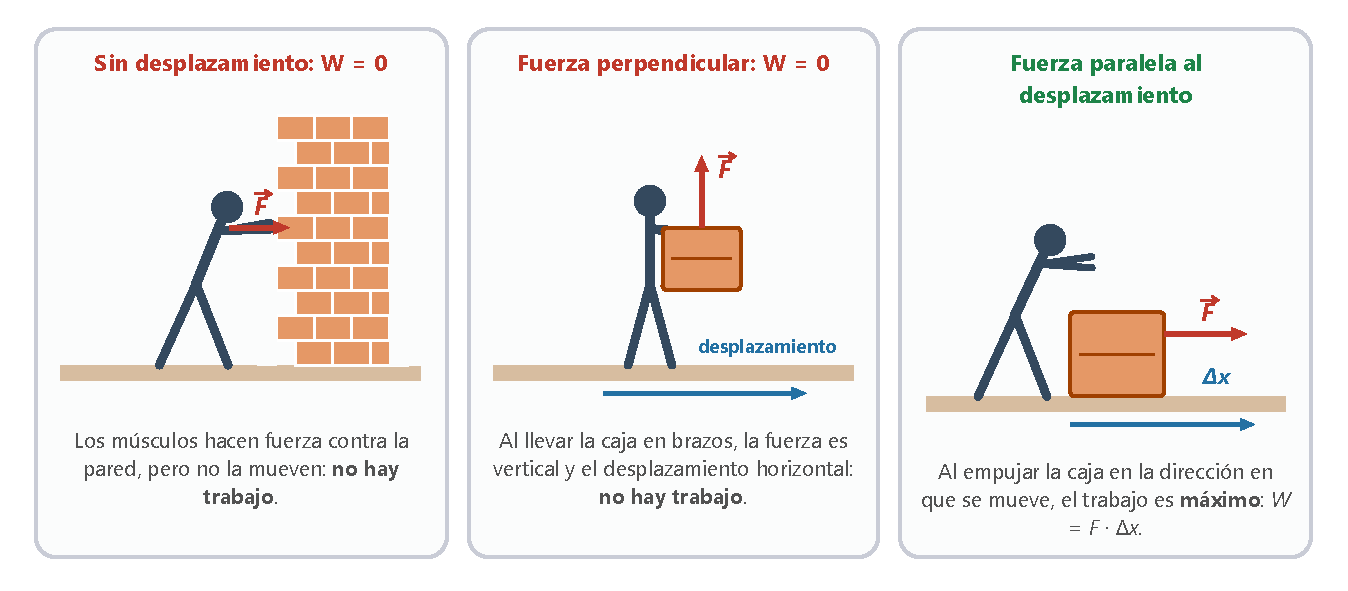
\includegraphics[width=\textwidth]{images/UD12/trabajo_casos}
    \caption{Solo hay trabajo si la fuerza produce un desplazamiento con una componente en su dirección.}
    \label{fig:ud12-casos}
\end{figure}

\subsection{Trabajo de una fuerza constante}

\begin{definition}[Trabajo mecánico]
    El trabajo que realiza una fuerza constante \(\vec{F}\) cuando su punto de aplicación se desplaza \(\Delta\vec{r}\) es el producto
    escalar de ambos vectores:
    \[ W = \vec{F} \cdot \Delta\vec{r} = F\,\Delta r\cos\alpha \]
    donde \(\alpha\) es el ángulo que forman la fuerza y el desplazamiento. Su unidad en el SI es el \textbf{julio} (J).
\end{definition}

\begin{itemize}
    \item \(\qty{1}{\joule}\) es el trabajo que hace una fuerza de \qty{1}{\newton} al desplazar su punto de aplicación \qty{1}{\m} en
    su misma dirección y sentido: \(\qty{1}{\joule} = \qty{1}{\newton\m} = \qty{1}{\kg\m\squared\per\s\squared}\).
    \item Es una magnitud \textbf{escalar}: no depende del sistema de coordenadas elegido.
    \item Solo trabaja la \textbf{componente de la fuerza paralela al desplazamiento}, \(F\cos\alpha\) (figura~\ref{fig:ud12-angulo}).
    \item El trabajo no depende del tiempo que se tarde en hacerlo.
\end{itemize}

\begin{remark}
    No hay que confundir \textbf{esfuerzo} con \textbf{trabajo}. Empujar una pared o sostener una maleta cansa mucho, porque los
    músculos consumen energía química, pero la fuerza que hacemos no realiza trabajo sobre la pared ni sobre la maleta, porque no las
    desplaza.
\end{remark}

\begin{figure}[H]
    \centering
    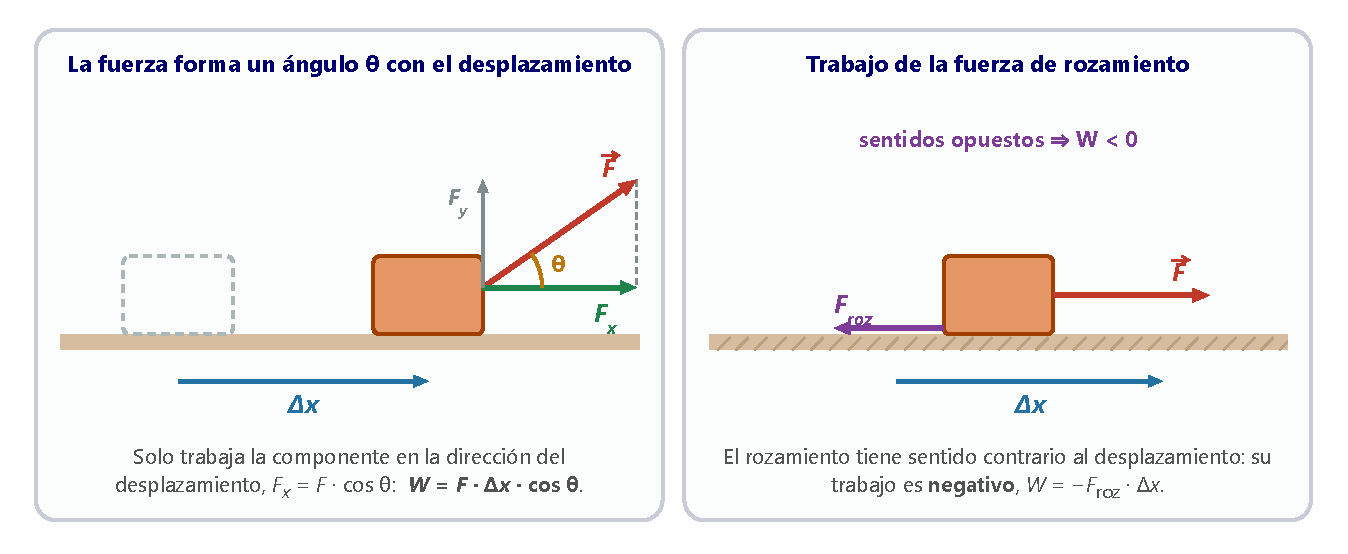
\includegraphics[width=\textwidth]{images/UD12/trabajo_angulo}
    \caption{Trabajo de una fuerza oblicua y de la fuerza de rozamiento.}
    \label{fig:ud12-angulo}
\end{figure}

\begin{example}
    \textbf{¿Hay trabajo?} Calcula el trabajo en estos casos: a) la fuerza con que sostenemos una mochila de \qty{8}{\kg} sin moverla;
    b) la fuerza gravitatoria que la Tierra ejerce sobre un satélite en órbita circular; c) una fuerza horizontal de \qty{10}{\newton}
    que desplaza \qty{60}{\cm} un carrito por un suelo horizontal.

    \textbf{Solución.} a) No hay desplazamiento: \(W = 0\). b) En una órbita circular, la fuerza gravitatoria apunta al centro y es
    siempre perpendicular al desplazamiento: \(W = F\,\Delta r\cos 90^\circ = 0\). c) \(W = 10 \cdot \num{0.6} \cdot \cos 0^\circ = \qty{6}{\joule}\).
\end{example}

\subsection{El signo del trabajo}

El signo del trabajo depende del ángulo entre la fuerza y el desplazamiento:

\begin{table}[H]
    \centering
    \caption{Signo del trabajo según el ángulo \(\alpha\) entre la fuerza y el desplazamiento}
    \vspace{-5pt}
    \begin{tabular}{@{}cL{11cm}@{}}
        \toprule
        \textbf{Ángulo} & \textbf{Trabajo} \\
        \midrule
        \(\alpha = 0^\circ\) & Fuerza y desplazamiento tienen la misma dirección y sentido: el trabajo es \textbf{máximo},
        \(W = F\,\Delta r\). \\[3pt]
        \(0^\circ \leq \alpha < 90^\circ\) & \(\cos\alpha > 0\): trabajo \textbf{positivo} o \textbf{motor}; la fuerza favorece el
        movimiento. \\[3pt]
        \(\alpha = 90^\circ\) & Fuerza perpendicular al desplazamiento: trabajo \textbf{nulo}. \\[3pt]
        \(90^\circ < \alpha \leq 180^\circ\) & \(\cos\alpha < 0\): trabajo \textbf{negativo} o \textbf{resistente}; la fuerza se opone
        al movimiento. \\
        \bottomrule
    \end{tabular}
    \label{tab:ud12-signo}
\end{table}

La \textbf{normal} y la \textbf{fuerza centrípeta} son ejemplos claros de trabajo nulo, porque son perpendiculares a la velocidad. El
\textbf{rozamiento cinético} sobre un cuerpo que desliza por una superficie fija se opone al deslizamiento, así que su trabajo es
negativo: \(W_r = -F_r\,\Delta r\).

\paragraph{Trabajo de varias fuerzas.} Si sobre un cuerpo actúan varias fuerzas, el \textbf{trabajo total} es la suma de los trabajos
de cada una, que coincide con el trabajo de la fuerza resultante:
\[ W_{\text{total}} = W_1 + W_2 + W_3 + \dots = \left(\sum \vec{F}\right) \cdot \Delta\vec{r} = F_{\text{neta}}\,\Delta r\cos\alpha \]

\begin{example}
    \textbf{El trabajo del peso en halterofilia.} Una halterófila levanta una barra de \qty{105}{\kg} hasta \qty{2.1}{\m} de altura.
    Calcula el trabajo que realiza el peso de la barra cuando: a) la barra sube \qty{2.1}{\m}; b) la deja caer y baja \qty{2.1}{\m};
    c) la barra rueda \qty{60}{\cm} por la tarima.

    \textbf{Solución.} \(P = 105 \cdot \num{9.8} = \qty{1029}{\newton}\).

    a) El peso apunta hacia abajo y la barra sube (\(\alpha = 180^\circ\)): \(W = 1029 \cdot \num{2.1} \cdot \cos 180^\circ = \qty{-2161}{\joule}\).
    Es un trabajo resistente.

    b) Peso y desplazamiento van hacia abajo (\(\alpha = 0^\circ\)): \(W = \qty{+2161}{\joule}\), un trabajo motor.

    c) El peso es perpendicular al desplazamiento horizontal: \(W = 0\).
\end{example}

\begin{exercise}
    Sobre una caja que se desliza por el suelo actúa una fuerza de \qty{90}{\newton}. Calcula su trabajo en un recorrido de \qty{12}{\m}
    si: a) tiene la dirección y el sentido del desplazamiento; b) forma \(45^\circ\) con él; c) es vertical hacia arriba; d) forma
    \(150^\circ\) con el desplazamiento.
    \begin{solu}
        a) \(\textcolor{red}{\qty{1080}{\joule}}\). b) \(90 \cdot 12 \cdot \cos 45^\circ = \textcolor{red}{\qty{764}{\joule}}\). c)
        \(\textcolor{red}{0}\). d) \(90 \cdot 12 \cdot \cos 150^\circ = \textcolor{red}{\qty{-935}{\joule}}\).
    \end{solu}
\end{exercise}

\begin{exercise}
    Un niño arrastra \qty{15}{\m} un trineo de \qty{20}{\kg} por un suelo horizontal tirando de una cuerda con una fuerza de
    \qty{60}{\newton} que forma \(30^\circ\) con la horizontal. El coeficiente de rozamiento es \num{0.1}. Calcula el trabajo de cada
    fuerza y el trabajo total.
    \begin{solu}
        \(W_F = 60 \cdot 15 \cdot \cos 30^\circ = \textcolor{red}{\qty{779}{\joule}}\); \(W_P = W_N = \textcolor{red}{0}\).
        \(N = 196 - 60\sen 30^\circ = \qty{166}{\newton}\); \(W_r = -\num{0.1} \cdot 166 \cdot 15 = \textcolor{red}{\qty{-249}{\joule}}\).
        \(W_{\text{total}} = \textcolor{red}{\qty{530}{\joule}}\).
    \end{solu}
\end{exercise}

\subsection{Interpretación gráfica del trabajo}

Si representamos la componente de la fuerza en la dirección del movimiento frente a la posición, el \textbf{trabajo es el área
comprendida entre la gráfica y el eje horizontal} (figura~\ref{fig:ud12-areas}). Esta idea permite calcular el trabajo de fuerzas
variables, como la de un muelle, para las que no sirve la expresión \(W = F\,\Delta x\cos\alpha\).

\begin{figure}[H]
    \centering
    \begin{tikzpicture}
        \begin{axis}[grafica, width=0.36\linewidth, height=4.2cm, xlabel={\(x\)}, ylabel={\(F\)}, xmin=0, xmax=6, ymin=0, ymax=5,
            xtick=\empty, ytick=\empty, title={\small Fuerza constante}]
            \addplot[fill=ocre!25, draw=none] coordinates {(1,0) (1,3) (5,3) (5,0)} \closedcycle;
            \addplot[very thick, ocre, domain=0:6] {3};
            \node[font=\small] at (axis cs:3,1.5) {\(W = F\,\Delta x\)};
        \end{axis}
    \end{tikzpicture}\hfill
    \begin{tikzpicture}
        \begin{axis}[grafica, width=0.36\linewidth, height=4.2cm, xlabel={\(x\)}, ylabel={\(F\)}, xmin=0, xmax=6, ymin=0, ymax=5,
            xtick=\empty, ytick=\empty, title={\small Fuerza elástica}]
            \addplot[fill=ocre!25, draw=none, domain=0:4.5] {0.9*x} \closedcycle;
            \addplot[very thick, ocre, domain=0:5.5] {0.9*x};
            \node[font=\small] at (axis cs:3.2,0.9) {\(W = \tfrac12 k\,x^2\)};
        \end{axis}
    \end{tikzpicture}\hfill
    \begin{tikzpicture}
        \begin{axis}[grafica, width=0.36\linewidth, height=4.2cm, xlabel={\(x\)}, ylabel={\(F\)}, xmin=0, xmax=6, ymin=0, ymax=5,
            xtick=\empty, ytick=\empty, title={\small Fuerza variable}]
            \addplot[fill=ocre!25, draw=none, domain=0.5:5, samples=50] {2+1.5*sin(deg(x-1))} \closedcycle;
            \addplot[very thick, ocre, domain=0:5.6, samples=50] {2+1.5*sin(deg(x-1))};
            \node[font=\small] at (axis cs:2.8,1.2) {\(W\) = área};
        \end{axis}
    \end{tikzpicture}
    \caption{El trabajo es el área bajo la gráfica fuerza-posición.}
    \label{fig:ud12-areas}
\end{figure}

\begin{example}
    \textbf{Una fuerza que deja de empujar.} Sobre un cuerpo actúa una fuerza paralela al desplazamiento que vale \qty{200}{\newton}
    durante los primeros \qty{3}{\m} y después disminuye uniformemente hasta anularse en \(x = \qty{5}{\m}\). ¿Qué trabajo realiza?

    \textbf{Solución.} El área bajo la gráfica es un rectángulo más un triángulo:
    \[ W = 200 \cdot 3 + \frac{1}{2} \cdot 200 \cdot 2 = 600 + 200 = \qty{800}{\joule} \]
\end{example}

\begin{exercise}
    Para estirar un muelle de constante \qty{400}{\newton\per\m} hay que hacer una fuerza \(F = k\,x\). Representa \(F\) frente al
    alargamiento y calcula, a partir de la gráfica, el trabajo necesario para estirarlo \qty{10}{\cm}.
    \begin{solu}
        Es el área de un triángulo de base \qty{0.1}{\m} y altura \(400 \cdot \num{0.1} = \qty{40}{\newton}\):
        \(W = \frac{1}{2} \cdot \num{0.1} \cdot 40 = \textcolor{red}{\qty{2}{\joule}}\).
    \end{solu}
\end{exercise}

%========================================================================================
\section{La energía cinética}\label{sec:ud12-cinetica}
%========================================================================================

Una nave que despega, una montaña rusa que se lanza cuesta abajo o una bola de bolos que derriba los bolos: todo cuerpo en movimiento
puede transformar su entorno. La palabra \textit{cinética} viene del griego \textit{kinetikós}, «que mueve».

\begin{definition}[Energía cinética]
    Es la energía que tiene un cuerpo por estar en movimiento. Para un cuerpo de masa \(m\) que se mueve con velocidad \(v\):
    \[ E_c = \frac{1}{2}\,m\,v^2 \]
\end{definition}

\begin{itemize}
    \item Es una magnitud \textbf{escalar}: depende del módulo de la velocidad, pero no de su dirección ni de su sentido.
    \item \textbf{Nunca es negativa}, porque \(m\) y \(v^2\) son siempre positivos.
    \item Depende del \textbf{cuadrado} de la velocidad: si la velocidad se duplica, la energía cinética se multiplica por cuatro.
    \item Se relaciona con el momento lineal, \(p = m\,v\): multiplicando y dividiendo por \(m\), \(E_c = \dfrac{m^2\,v^2}{2\,m} = \dfrac{p^2}{2\,m}\).
\end{itemize}

\begin{example}
    \textbf{Pruebas de choque.} En unas pruebas de choque se lanza un coche de \qty{1400}{\kg} a \qty{90}{\km\per\hour} y un camión de
    \qty{3600}{\kg} a \qty{15}{\m\per\s}. ¿Cuál tiene más energía cinética?

    \textbf{Solución.} Pasamos la velocidad del coche al SI: \(\qty{90}{\km\per\hour} = \dfrac{90\,000}{3600} = \qty{25}{\m\per\s}\).
    \[ E_{c,\text{coche}} = \frac{1}{2} \cdot 1400 \cdot 25^2 = \qty{4.38e5}{\joule} \qquad
    E_{c,\text{camión}} = \frac{1}{2} \cdot 3600 \cdot 15^2 = \qty{4.05e5}{\joule} \]
    El coche tiene más energía cinética, aunque su masa es mucho menor: la velocidad influye al cuadrado.
\end{example}

\subsection{Teorema de las fuerzas vivas}

El trabajo y la energía cinética se miden en la misma unidad. Veamos qué relación hay entre ellos en un caso sencillo: un cuerpo de
masa \(m\) que se mueve en línea recta empujado por una fuerza neta constante \(F\) en el sentido del movimiento. El trabajo de esa
fuerza es \(W = F\,\Delta x = m\,a\,\Delta x\). En un MRUA, \(v^2 = v_0^2 + 2\,a\,\Delta x\), así que \(a\,\Delta x = \dfrac{v^2 - v_0^2}{2}\):
\[ W = m\,\frac{v^2 - v_0^2}{2} = \frac{1}{2}\,m\,v^2 - \frac{1}{2}\,m\,v_0^2 = E_{c,f} - E_{c,i} \]
Este resultado es general; lo enunció Gaspard-Gustave \textbf{Coriolis} hacia 1829, a partir de las ideas de Galileo y Leibniz.

\begin{definition}[Teorema de las fuerzas vivas o de la energía cinética]
    El trabajo total realizado sobre un cuerpo (el de todas las fuerzas que actúan sobre él) es igual a la variación de su energía
    cinética:
    \[ W_{\text{total}} = \Delta E_c = E_{c,f} - E_{c,i} \]
\end{definition}

\begin{itemize}
    \item Si \(W_{\text{total}} > 0\), la energía cinética \textbf{aumenta}: el cuerpo acelera.
    \item Si \(W_{\text{total}} < 0\), la energía cinética \textbf{disminuye}: el cuerpo frena.
    \item Si \(W_{\text{total}} = 0\), la energía cinética \textbf{no cambia} (por ejemplo, en un MCU).
\end{itemize}

\begin{figure}[H]
    \centering
    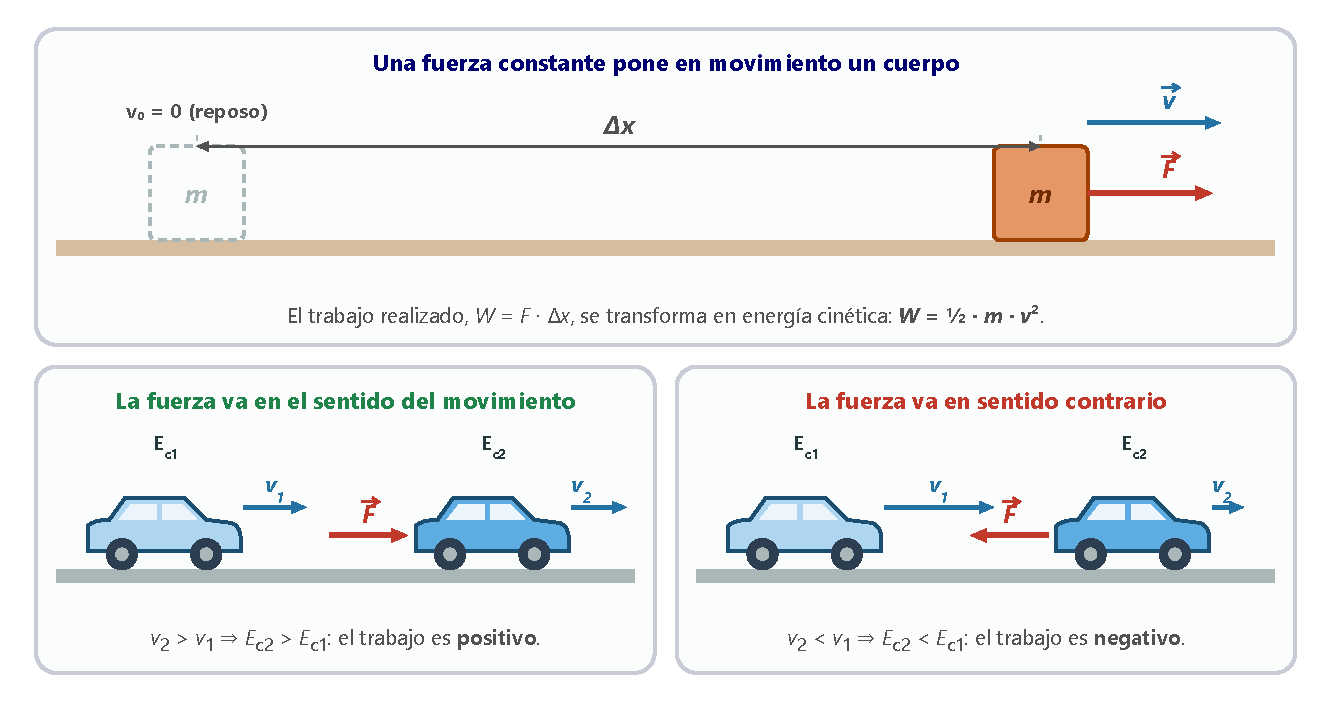
\includegraphics[width=\textwidth]{images/UD12/energia_cinetica}
    \caption{El trabajo de la fuerza neta se invierte en cambiar la energía cinética.}
    \label{fig:ud12-cinetica}
\end{figure}

\begin{remark}
    El trabajo \textbf{no es una forma de energía}, sino una manera de \textbf{transferir} energía de un sistema a otro. Un cuerpo
    tiene energía, pero no «tiene trabajo».
\end{remark}

\begin{example}
    \textbf{Un control de velocidad.} Un coche de \qty{1100}{\kg} circula a \qty{110}{\km\per\hour}, ve un radar y frena hasta
    \qty{80}{\km\per\hour}. ¿Cuánto ha variado su energía cinética? ¿Qué trabajo han hecho los frenos?

    \textbf{Solución.} \(v_i = \qty{30.6}{\m\per\s}\), \(v_f = \qty{22.2}{\m\per\s}\).
    \[ E_{c,i} = \frac{1}{2} \cdot 1100 \cdot \num{30.56}^2 = \qty{5.14e5}{\joule} \qquad E_{c,f} = \frac{1}{2} \cdot 1100 \cdot \num{22.22}^2
    = \qty{2.72e5}{\joule} \]
    \(\Delta E_c = \qty{-2.42e5}{\joule}\). Por el teorema de las fuerzas vivas, el trabajo de los frenos (y demás fuerzas resistentes)
    es \(W = \qty{-2.42e5}{\joule}\); esa energía acaba como calor en los discos de freno.
\end{example}

\begin{example}
    \textbf{Un carro de reparto.} Un repartidor tira de un carro de \qty{18}{\kg}, que parte del reposo, con una fuerza de
    \qty{50}{\newton} que forma \(30^\circ\) con la horizontal, a lo largo de \qty{8}{\m}. Despreciando el rozamiento, calcula: a) el
    trabajo de cada fuerza; b) la velocidad final del carro.

    \textbf{Solución.} a) Sobre el carro actúan el peso, la normal y la fuerza del repartidor. El peso y la normal son perpendiculares al
    desplazamiento: \(W_P = W_N = 0\). Solo trabaja la fuerza aplicada: \(W_F = 50 \cdot 8 \cdot \cos 30^\circ = \qty{346}{\joule}\).

    b) Por el teorema de las fuerzas vivas, \(W_{\text{total}} = \frac{1}{2}\,m\,v^2 - 0\):
    \[ v = \sqrt{\frac{2\,W}{m}} = \sqrt{\frac{2 \cdot 346}{18}} = \qty{6.20}{\m\per\s} \]
\end{example}

\begin{exercise}
    Un velocista de \qty{80}{\kg} alcanza una velocidad máxima de \qty{12}{\m\per\s} en una carrera de \qty{100}{\m}. ¿Qué energía
    cinética tiene en ese momento?
    \begin{solu}
        \(E_c = \frac{1}{2} \cdot 80 \cdot 12^2 = \textcolor{red}{\qty{5760}{\joule}}\).
    \end{solu}
\end{exercise}

\begin{exercise}
    En una partida de \textit{air hockey}, el disco, de \qty{40}{\g}, pasa de \qty{10}{\m\per\s} a \qty{15}{\m\per\s} tras un golpe.
    ¿Qué trabajo ha realizado el mazo sobre el disco?
    \begin{solu}
        \(W = \Delta E_c = \frac{1}{2} \cdot \num{0.04} \cdot (15^2 - 10^2) = \textcolor{red}{\qty{2.5}{\joule}}\).
    \end{solu}
\end{exercise}

\begin{exercise}
    En la salida de una carrera, una moto y su piloto, de \qty{220}{\kg} en total, alcanzan \qty{162}{\km\per\hour} en un tramo de
    \qty{180}{\m}. Calcula la variación de su energía cinética y la fuerza neta media que actúa sobre la moto.
    \begin{solu}
        \(v = \qty{45}{\m\per\s}\): \(\Delta E_c = \frac{1}{2} \cdot 220 \cdot 45^2 = \textcolor{red}{\qty{2.23e5}{\joule}}\);
        \(F = \dfrac{\Delta E_c}{\Delta x} = \textcolor{red}{\qty{1238}{\newton}}\).
    \end{solu}
\end{exercise}

\begin{exercise}
    Un balón de \qty{450}{\g} tiene un momento lineal de \qty{9}{\kg\m\per\s}. Calcula su energía cinética sin calcular antes la
    velocidad. Comprueba el resultado calculando la velocidad.
    \begin{solu}
        \(E_c = \dfrac{p^2}{2\,m} = \dfrac{81}{\num{0.9}} = \textcolor{red}{\qty{90}{\joule}}\); \(v = \dfrac{9}{\num{0.45}} = \qty{20}{\m\per\s}\)
        y \(\frac{1}{2} \cdot \num{0.45} \cdot 20^2 = \qty{90}{\joule}\).
    \end{solu}
\end{exercise}

%========================================================================================
\section{Fuerzas conservativas y energía potencial}\label{sec:ud12-potencial}
%========================================================================================

Una roca en el borde de un acantilado o el muelle comprimido de una lanzadora de paintball no se mueven, pero pueden hacerlo: tienen
energía almacenada por su \textbf{posición} o su \textbf{configuración}. El término \textit{energía potencial} lo introdujo el ingeniero
escocés William Rankine a mediados del siglo \textsc{xix}.

\subsection{Fuerzas conservativas}

\begin{definition}[Fuerza conservativa]
    Una fuerza es conservativa si el trabajo que realiza sobre un cuerpo que pasa de un punto a otro depende solo de las posiciones
    inicial y final, y no del camino seguido. De forma equivalente: su trabajo a lo largo de cualquier trayectoria cerrada es nulo.
\end{definition}

El \textbf{peso} es una fuerza conservativa: tanto si un cuerpo cae en vertical como si baja por un plano inclinado o describe una
parábola, el trabajo del peso es \(m\,g\,h\), donde \(h\) es la diferencia de alturas (figura~\ref{fig:ud12-caminos}). También son
conservativas la \textbf{fuerza elástica} de un muelle, la \textbf{gravitatoria} y la \textbf{electrostática}. El \textbf{rozamiento}, en
cambio, \textbf{no es conservativo}: cuanto más largo es el camino, más trabajo (negativo) realiza. Tampoco lo son, en general, las
fuerzas que aplicamos con las manos o con un motor.

\begin{figure}[H]
    \centering
    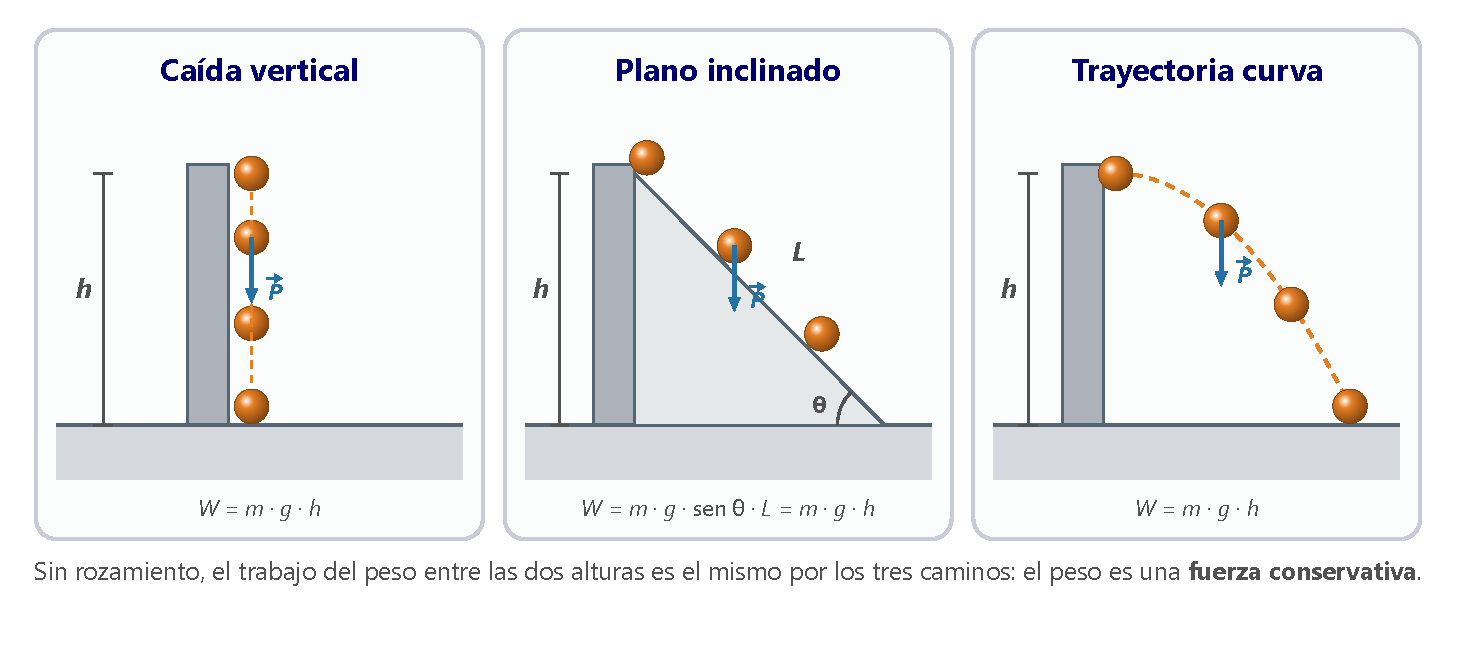
\includegraphics[width=\textwidth]{images/UD12/caminos_peso}
    \caption{El trabajo del peso entre dos alturas no depende del camino.}
    \label{fig:ud12-caminos}
\end{figure}

Como el trabajo de una fuerza conservativa solo depende de los puntos inicial y final, se le puede asociar una función de la posición,
la \textbf{energía potencial}, \(E_p\), de modo que:

\begin{definition}[Energía potencial]
    Es la energía que tiene un cuerpo por su posición o configuración en un campo de fuerzas conservativas. El trabajo de una fuerza
    conservativa es igual a la variación de la energía potencial cambiada de signo:
    \[ W_{\text{cons}} = -\Delta E_p = -(E_{p,f} - E_{p,i}) = E_{p,i} - E_{p,f} \]
\end{definition}

Solo las fuerzas conservativas tienen asociada una energía potencial. Si la fuerza conservativa realiza un trabajo positivo (por
ejemplo, el peso cuando un cuerpo cae), la energía potencial disminuye. Un sistema tiende de forma natural hacia la posición de
\textbf{mínima energía potencial}: una piedra cae, un muelle estirado vuelve a su longitud natural.

\subsection{Energía potencial gravitatoria}

Calculemos el trabajo del peso cuando un cuerpo sube desde una altura \(h_i\) hasta una altura \(h_f\). El peso apunta hacia abajo y
el desplazamiento, hacia arriba:
\[ W_{\text{peso}} = m\,g\,(h_f - h_i)\cos 180^\circ = m\,g\,h_i - m\,g\,h_f \]
Comparando con \(W_{\text{cons}} = E_{p,i} - E_{p,f}\), la energía potencial gravitatoria es:

\begin{definition}[Energía potencial gravitatoria]
    Es la energía que tiene un cuerpo de masa \(m\) situado a una altura \(h\) sobre un nivel de referencia, cerca de la superficie
    terrestre:
    \[ E_p = m\,g\,h \]
\end{definition}

\begin{itemize}
    \item Solo vale para \textbf{alturas pequeñas} comparadas con el radio terrestre, donde \(g\) es constante. Para alturas grandes
    hay que usar la ley de la gravitación universal (lo estudiarás en 2.º de Bachillerato).
    \item Su valor depende del \textbf{nivel de referencia} (\(h = 0\)), que elegimos libremente: puede ser positiva o negativa
    (un cuerpo en el fondo de un pozo tiene \(E_p < 0\) si tomamos como referencia el suelo).
    \item Lo que tiene sentido físico es la \textbf{variación} de energía potencial, que no depende del nivel de referencia.
\end{itemize}

\begin{figure}[H]
    \centering
    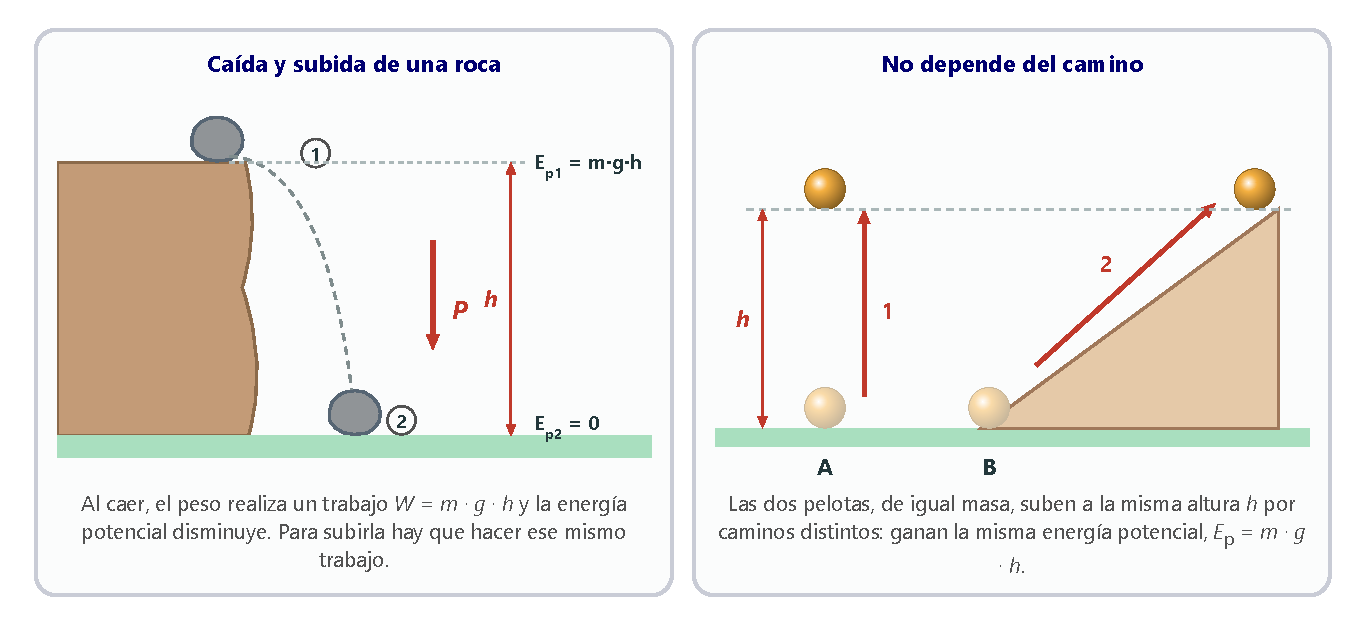
\includegraphics[width=\textwidth]{images/UD12/energia_potencial}
    \caption{La energía potencial gravitatoria depende solo de la altura.}
    \label{fig:ud12-potencial}
\end{figure}

\begin{remark}
    El agua de un embalse tiene energía potencial gravitatoria. En una \textbf{central hidroeléctrica}, el agua cae por unas tuberías
    y mueve las turbinas: su energía potencial se transforma en cinética y después en eléctrica. Es una fuente renovable.
\end{remark}

\begin{example}
    \textbf{Un gato en el balcón.} Un gato de \qty{4}{\kg} está sobre la barandilla de un balcón, a \qty{1}{\m} del suelo del balcón,
    que está a \qty{6}{\m} sobre la calle. a) Calcula su energía potencial respecto al suelo del balcón y respecto a la calle. b) Si salta
    al suelo del balcón, ¿qué trabajo realiza el peso?

    \textbf{Solución.} a) Respecto al balcón: \(E_p = 4 \cdot \num{9.8} \cdot 1 = \qty{39.2}{\joule}\). Respecto a la calle:
    \(E_p = 4 \cdot \num{9.8} \cdot 7 = \qty{274.4}{\joule}\).

    b) \(W = -\Delta E_p\). Con la referencia en el balcón: \(W = -(0 - \num{39.2}) = \qty{39.2}{\joule}\). Con la referencia en la
    calle: \(W = -(4 \cdot \num{9.8} \cdot 6 - \num{274.4}) = \qty{39.2}{\joule}\). El trabajo no depende del nivel de referencia.
\end{example}

\begin{exercise}
    Una persona de \qty{65}{\kg} sube desde la planta baja hasta un cuarto piso; cada planta mide \qty{3}{\m}. ¿Cuánto aumenta su
    energía potencial? ¿Qué trabajo hace el peso?
    \begin{solu}
        \(\Delta E_p = 65 \cdot \num{9.8} \cdot 12 = \textcolor{red}{\qty{7644}{\joule}}\); \(W_{\text{peso}} = \textcolor{red}{\qty{-7644}{\joule}}\).
    \end{solu}
\end{exercise}

\begin{exercise}
    Se deja caer una moneda de \qty{7.5}{\g} desde un mirador situado a \qty{250}{\m} de altura. Despreciando el rozamiento con el
    aire, calcula: a) su energía potencial inicial; b) su energía potencial cuando está a \qty{125}{\m} del suelo; c) su velocidad y su
    energía cinética en ese punto; d) la suma de las energías de b) y c). Explica el resultado.
    \begin{solu}
        a) \(\textcolor{red}{\qty{18.4}{\joule}}\). b) \(\textcolor{red}{\qty{9.19}{\joule}}\). c) \(v = \sqrt{2 \cdot \num{9.8} \cdot 125}
        = \textcolor{red}{\qty{49.5}{\m\per\s}}\); \(E_c = \textcolor{red}{\qty{9.19}{\joule}}\). d) \(\textcolor{red}{\qty{18.4}{\joule}}\):
        la energía potencial perdida se ha convertido en cinética y la suma no cambia. (En realidad, el rozamiento del aire limitaría
        mucho la velocidad).
    \end{solu}
\end{exercise}

\begin{exercise}
    Calcula la energía potencial de una roca de \qty{400}{\kg} en lo alto de un cerro de \qty{120}{\m} respecto a su base.
    \begin{solu}
        \(E_p = 400 \cdot \num{9.8} \cdot 120 = \textcolor{red}{\qty{4.70e5}{\joule}}\).
    \end{solu}
\end{exercise}

\subsection{Energía potencial elástica}

Para estirar o comprimir un muelle hay que aplicar una fuerza igual y opuesta a la recuperadora: según la ley de Hooke,
\(F_{\text{ext}} = k\,x\), donde \(x\) es la deformación respecto a la posición de equilibrio. Como la fuerza crece con la deformación,
el trabajo necesario es el área del triángulo de la gráfica \(F\)-\(x\): \(\frac{1}{2}\,x \cdot k\,x\). Ese trabajo queda
almacenado en el muelle (figura~\ref{fig:ud12-muelle}).

\begin{definition}[Energía potencial elástica]
    Es la energía almacenada en un cuerpo elástico deformado, como un muelle o una goma. Tomando como referencia la posición de
    equilibrio (\(x = 0\)):
    \[ E_{p,\text{elást}} = \frac{1}{2}\,k\,x^2 \]
    donde \(k\) es la constante elástica y \(x\) la deformación (alargamiento o compresión).
\end{definition}

\begin{figure}[H]
    \centering
    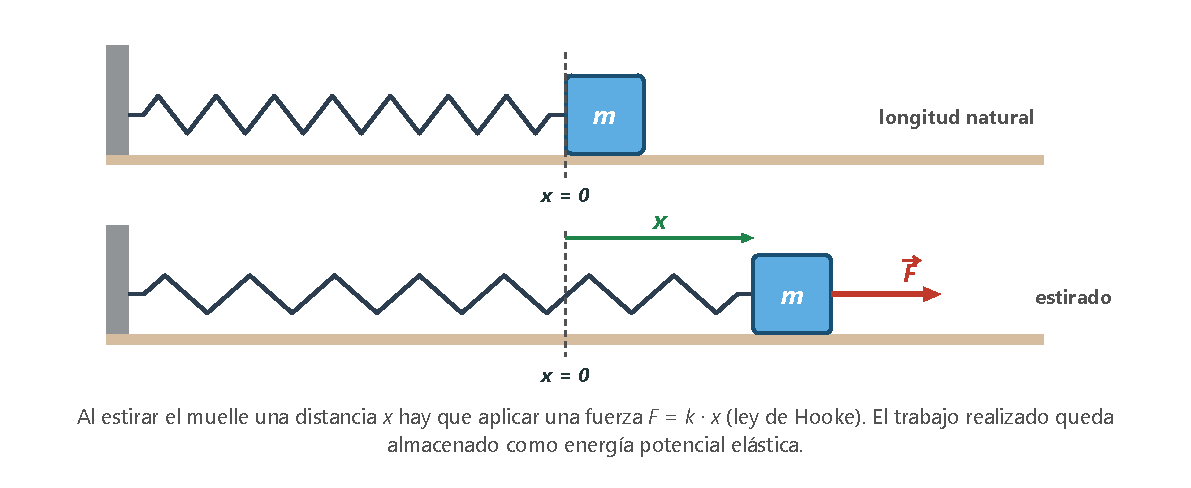
\includegraphics[width=0.85\textwidth]{images/UD12/muelle}
    \caption{Un muelle estirado almacena energía potencial elástica.}
    \label{fig:ud12-muelle}
\end{figure}

\begin{itemize}
    \item Es \textbf{siempre positiva}, tanto si el muelle se estira (\(x > 0\)) como si se comprime (\(x < 0\)), porque depende de
    \(x^2\) (figura~\ref{fig:ud12-parabola}).
    \item El trabajo de la fuerza elástica, que es conservativa, es \(W_{\text{elást}} = -\Delta E_p = \frac{1}{2}\,k\,(x_i^2 - x_f^2)\).
    \item El trabajo de la fuerza exterior que deforma el muelle es igual pero de signo contrario: \(W_{\text{ext}} = \Delta E_p\).
\end{itemize}

\begin{figure}[H]
    \centering
    \begin{tikzpicture}
        \begin{axis}[grafica, width=0.6\linewidth, height=5cm, xlabel={\(x\)}, ylabel={}, xmin=-3, xmax=3, ymin=-3.2, ymax=4.6,
            xtick=\empty, ytick=\empty, axis lines=middle]
            \addplot[very thick, ocre, domain=-2.9:2.9, samples=60] {0.5*x^2};
            \addplot[very thick, blue!60!black, domain=-2.9:2.9] {-x};
            \node[font=\small, ocre] at (axis cs:2.15,4.1) {\(E_p = \tfrac12 k\,x^2\)};
            \node[font=\small, blue!60!black] at (axis cs:2.25,-2.7) {\(F = -k\,x\)};
            \node[font=\scriptsize, align=center] at (axis cs:-1.9,0.4) {compresión};
            \node[font=\scriptsize, align=center] at (axis cs:1.9,0.4) {alargamiento};
        \end{axis}
    \end{tikzpicture}
    \caption{Energía potencial elástica y fuerza recuperadora de un muelle frente a la deformación.}
    \label{fig:ud12-parabola}
\end{figure}

\begin{example}
    \textbf{Una pista de coches de juguete.} En la rampa de lanzamiento de una pista se coloca un coche de \qty{30}{\g} comprimiendo
    \qty{4}{\cm} un muelle de constante \qty{80}{\newton\per\m}. Calcula la energía potencial del muelle y la velocidad con que sale el
    coche si recibe toda esa energía.

    \textbf{Solución.} \(E_p = \frac{1}{2} \cdot 80 \cdot \num{0.04}^2 = \qty{0.064}{\joule}\). Si toda se transforma en energía cinética:
    \[ \frac{1}{2}\,m\,v^2 = E_p \Rightarrow v = \sqrt{\frac{2 \cdot \num{0.064}}{\num{0.03}}} = \qty{2.07}{\m\per\s} \]
\end{example}

\begin{exercise}
    De un muelle de constante \qty{300}{\newton\per\m} se cuelga primero una masa de \qty{2}{\kg} y después otra de \qty{4}{\kg}.
    ¿Cuánto se estira y qué energía potencial elástica almacena en cada caso?
    \begin{solu}
        \(x = \dfrac{m\,g}{k}\): \(\textcolor{red}{\qty{6.5}{\cm}}\) y \(\textcolor{red}{\qty{0.64}{\joule}}\); \(\textcolor{red}{\qty{13.1}{\cm}}\)
        y \(\textcolor{red}{\qty{2.56}{\joule}}\). Al duplicar la masa, la energía se multiplica por cuatro.
    \end{solu}
\end{exercise}

\begin{exercise}
    Al colgar una masa de \qty{600}{\g} de un muelle, este se estira \qty{3}{\cm}. Calcula su constante elástica y la energía que
    almacena.
    \begin{solu}
        \(k = \dfrac{\num{0.6} \cdot \num{9.8}}{\num{0.03}} = \textcolor{red}{\qty{196}{\newton\per\m}}\);
        \(E_p = \frac{1}{2} \cdot 196 \cdot \num{0.03}^2 = \textcolor{red}{\qty{0.088}{\joule}}\).
    \end{solu}
\end{exercise}

\begin{exercise}
    En una caja sorpresa hay dos muñecos, cada uno sobre un muelle de constante \qty{120}{\newton\per\m} comprimido \qty{6}{\cm}. ¿Qué
    energía potencial elástica almacena el conjunto antes de abrir la caja?
    \begin{solu}
        \(E_p = 2 \cdot \frac{1}{2} \cdot 120 \cdot \num{0.06}^2 = \textcolor{red}{\qty{0.43}{\joule}}\).
    \end{solu}
\end{exercise}

\paragraph{Otras formas de energía potencial.} La \textbf{energía química} es energía potencial almacenada en los enlaces entre
átomos: se libera en una combustión y se almacena en la fotosíntesis. La \textbf{energía potencial eléctrica} aparece entre cuerpos
con carga: en una tormenta, un rayo puede liberar del orden de \(10^9\)~J. La \textbf{energía nuclear} es energía potencial asociada a
las fuerzas que mantienen unidos los protones y neutrones del núcleo; se libera en la fisión y en la fusión.

%========================================================================================
\section{Conservación de la energía mecánica}\label{sec:ud12-conservacion}
%========================================================================================

\begin{definition}[Energía mecánica]
    Es la suma de la energía cinética y de todas las formas de energía potencial de un cuerpo:
    \[ E_m = E_c + E_p \]
\end{definition}

Reunamos lo que sabemos: el trabajo total sobre un cuerpo es igual a la variación de su energía cinética, \(W_{\text{total}} = \Delta E_c\),
y el trabajo de las fuerzas conservativas es \(W_{\text{cons}} = -\Delta E_p\).

\subsection{Teorema de conservación de la energía mecánica}

Supongamos que solo realizan trabajo fuerzas conservativas (porque no hay otras o porque, como la normal, no trabajan). Entonces
\(W_{\text{total}} = W_{\text{cons}}\), es decir:
\[ \Delta E_c = -\Delta E_p \Rightarrow E_{c,f} - E_{c,i} = E_{p,i} - E_{p,f} \Rightarrow E_{c,f} + E_{p,f} = E_{c,i} + E_{p,i} \]

\begin{definition}[Teorema de conservación de la energía mecánica]
    Si sobre un sistema solo realizan trabajo fuerzas conservativas, su energía mecánica permanece constante:
    \[ W_{\text{no cons}} = 0 \Rightarrow E_m = E_c + E_p = \text{constante} \]
\end{definition}

La energía mecánica no cambia, pero sus componentes sí: lo que gana la energía cinética lo pierde la potencial, y viceversa
(\(\Delta E_c = -\Delta E_p\)). Es lo que ocurre en un tobogán, en un columpio o en una montaña rusa sin rozamiento
(figura~\ref{fig:ud12-conservacion}).

\begin{figure}[H]
    \centering
    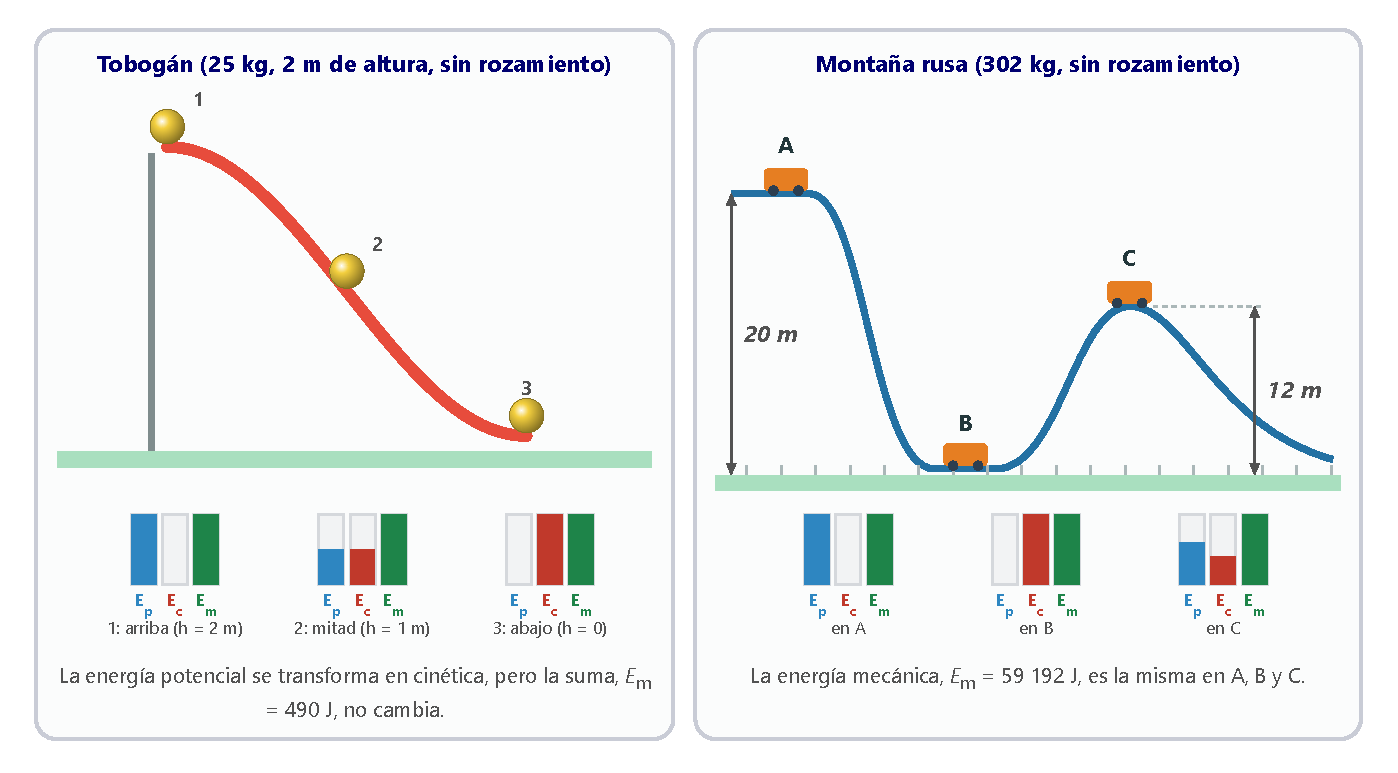
\includegraphics[width=\textwidth]{images/UD12/conservacion}
    \caption{Conservación de la energía mecánica en un tobogán y en una montaña rusa.}
    \label{fig:ud12-conservacion}
\end{figure}

\begin{figure}[H]
    \centering
    \begin{tikzpicture}
        \begin{axis}[grafica, width=0.6\linewidth, height=5cm, xlabel={altura, \(h\)}, ylabel={Energía}, xmin=0, xmax=10.5, ymin=0,
            ymax=12, xtick={0,10}, xticklabels={0,\(h_0\)}, ytick=\empty, legend pos=outer north east, legend style={font=\small}]
            \addplot[very thick, ocre, domain=0:10] {x}; \addlegendentry{\(E_p\)}
            \addplot[very thick, blue!60!black, domain=0:10] {10-x}; \addlegendentry{\(E_c\)}
            \addplot[very thick, dashed, green!50!black, domain=0:10] {10}; \addlegendentry{\(E_m\)}
        \end{axis}
    \end{tikzpicture}
    \caption{Energías de un cuerpo que cae desde una altura \(h_0\) sin rozamiento: la mecánica se mantiene constante.}
    \label{fig:ud12-caida}
\end{figure}

\begin{example}
    \textbf{En el \textit{half-pipe}.} Una patinadora de \qty{55}{\kg} llega al borde de una rampa en U (\textit{half-pipe}) con
    \qty{4}{\m\per\s}. ¿Con qué velocidad pasará por el fondo, \qty{3.5}{\m} más abajo, si no hay rozamiento?

    \textbf{Solución.} Solo trabaja el peso (la normal es perpendicular a la pista): la energía mecánica se conserva. Tomando el fondo
    como referencia:
    \[ \frac{1}{2}\,m\,v_1^2 + m\,g\,h = \frac{1}{2}\,m\,v_2^2 \Rightarrow v_2 = \sqrt{v_1^2 + 2\,g\,h} = \sqrt{16 + 2 \cdot \num{9.8} \cdot \num{3.5}}
    = \qty{9.20}{\m\per\s} \]
    La masa se simplifica: el resultado no depende de ella.
\end{example}

\begin{example}
    \textbf{Caída sobre un muelle.} Desde \qty{60}{\cm} por encima de un muelle vertical de constante \qty{20}{\newton\per\m} se suelta
    un cuerpo de \qty{40}{\g}. ¿Cuánto se comprime el muelle?

    \textbf{Solución.} Tomamos como referencia de alturas el punto de máxima compresión, \(x\) por debajo del extremo del muelle. Al
    principio y al final el cuerpo está en reposo, así que toda la energía potencial gravitatoria se transforma en elástica:
    \[ m\,g\,(\num{0.6} + x) = \frac{1}{2}\,k\,x^2 \Rightarrow \num{0.392} \cdot (\num{0.6} + x) = 10\,x^2 \Rightarrow 10\,x^2 - \num{0.392}\,x - \num{0.235} = 0 \]
    La solución positiva es \(x = \qty{0.174}{\m} = \qty{17.4}{\cm}\).
\end{example}

\begin{exercise}
    Un escalador resbala y cae desde \qty{5}{\m} hasta la colchoneta. ¿Con qué velocidad llega, si despreciamos el rozamiento con el aire?
    \begin{solu}
        \(v = \sqrt{2\,g\,h} = \textcolor{red}{\qty{9.90}{\m\per\s}}\).
    \end{solu}
\end{exercise}

\begin{exercise}
    Una montaña rusa empieza con una gran bajada. ¿Desde qué altura parte, en reposo, el vagón si llega al punto más bajo a
    \qty{30}{\m\per\s}? Desprecia el rozamiento. ¿Influye que el vagón vaya lleno o vacío?
    \begin{solu}
        \(h = \dfrac{v^2}{2\,g} = \textcolor{red}{\qty{45.9}{\m}}\). \textcolor{red}{No influye}: la masa se simplifica.
    \end{solu}
\end{exercise}

\subsection{Fuerzas no conservativas: la energía disipada}

En general, sobre un cuerpo actúan fuerzas conservativas y no conservativas (rozamiento, fuerzas aplicadas, motores):
\[ W_{\text{total}} = W_{\text{cons}} + W_{\text{no cons}} \Rightarrow \Delta E_c = -\Delta E_p + W_{\text{no cons}} \]

\begin{definition}[Trabajo de las fuerzas no conservativas]
    El trabajo de las fuerzas no conservativas es igual a la variación de la energía mecánica:
    \[ W_{\text{no cons}} = \Delta E_m = E_{m,f} - E_{m,i} \]
\end{definition}

\begin{itemize}
    \item Si \(W_{\text{no cons}} > 0\), la energía mecánica \textbf{aumenta} (un motor, una persona que empuja).
    \item Si \(W_{\text{no cons}} < 0\), la energía mecánica \textbf{disminuye}. La energía perdida o \textbf{disipada} se transforma
    en otras formas menos útiles, sobre todo en energía térmica por el rozamiento.
\end{itemize}

La energía total (mecánica más térmica y demás formas) sigue conservándose: el \textbf{principio de conservación de la energía} se cumple
siempre (figura~\ref{fig:ud12-rozamiento}). Lo que ocurre es que la energía se \textbf{degrada}.

\begin{figure}[H]
    \centering
    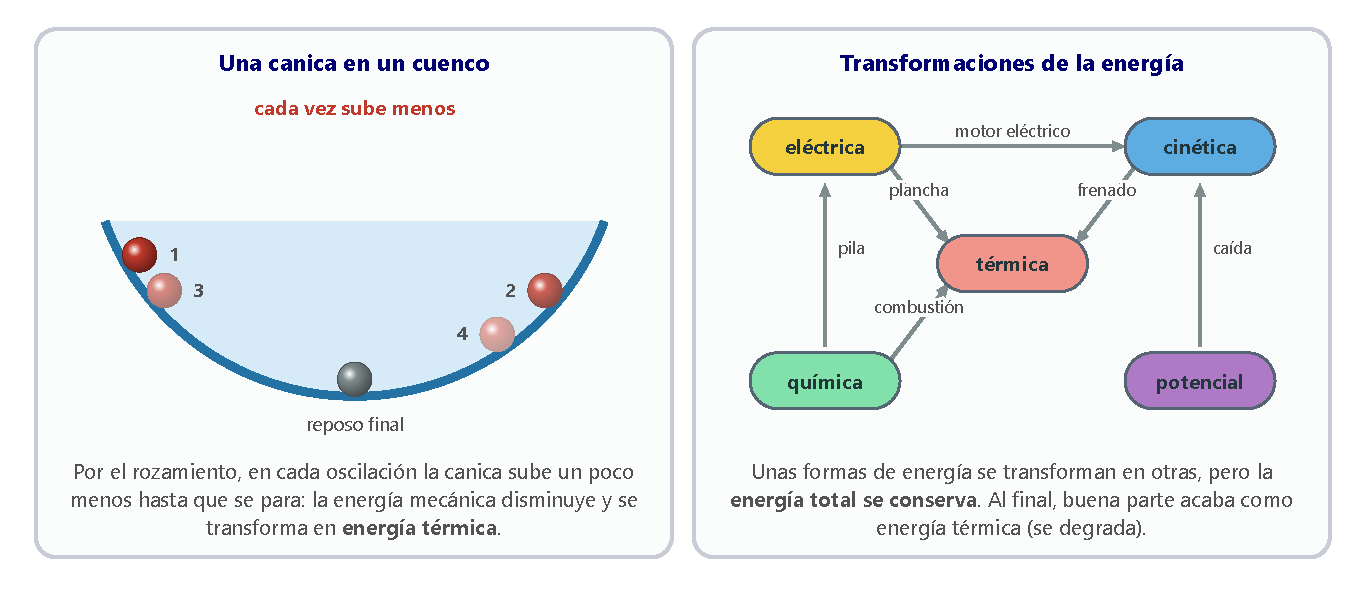
\includegraphics[width=\textwidth]{images/UD12/rozamiento_energia}
    \caption{El rozamiento transforma energía mecánica en térmica; la energía total se conserva.}
    \label{fig:ud12-rozamiento}
\end{figure}

\begin{remark}
    La ecuación de Einstein, \(E = m\,c^2\), muestra que la masa también es una forma de energía. En las reacciones nucleares, una
    pequeña parte de la masa se transforma en una enorme cantidad de energía.
\end{remark}

\begin{example}
    \textbf{El trabajo del motor.} Un coche de \qty{1200}{\kg} arranca y acelera a razón de \qty{2.5}{\m\per\s\squared} durante
    \qty{8}{\s} por una carretera horizontal. Las fuerzas de resistencia (aire y rodadura) equivalen a un coeficiente de rozamiento de
    \num{0.05}. Calcula el trabajo de las fuerzas de resistencia y el del motor.

    \textbf{Solución.} Cinemática: \(x = \frac{1}{2} \cdot \num{2.5} \cdot 8^2 = \qty{80}{\m}\); \(v = \num{2.5} \cdot 8 = \qty{20}{\m\per\s}\).

    Resistencias: \(W_r = -\mu\,m\,g\,x = -\num{0.05} \cdot 1200 \cdot \num{9.8} \cdot 80 = \qty{-4.70e4}{\joule}\).

    La carretera es horizontal, así que la energía mecánica es solo cinética: \(W_{\text{no cons}} = W_{\text{motor}} + W_r = \Delta E_c\):
    \[ W_{\text{motor}} = \frac{1}{2} \cdot 1200 \cdot 20^2 - (\num{-4.70e4}) = \num{2.40e5} + \num{4.70e4} = \qty{2.87e5}{\joule} \]
\end{example}

\begin{exercise}
    Un cuerpo de \qty{12}{\kg} parte del reposo en lo alto de un plano inclinado \(30^\circ\) y de \qty{6}{\m} de longitud. Calcula su
    velocidad al llegar abajo: a) sin rozamiento; b) si actúa una fuerza de rozamiento de \qty{20}{\newton}.
    \begin{solu}
        \(h = 6 \cdot \sen 30^\circ = \qty{3}{\m}\). a) \(v = \sqrt{2\,g\,h} = \textcolor{red}{\qty{7.67}{\m\per\s}}\). b)
        \(W_r = -20 \cdot 6 = \qty{-120}{\joule}\); \(E_c = \num{352.8} - 120 = \qty{232.8}{\joule}\); \(v = \textcolor{red}{\qty{6.23}{\m\per\s}}\).
    \end{solu}
\end{exercise}

\begin{exercise}
    Un esquiador de \qty{80}{\kg} empieza a bajar a \qty{5}{\m\per\s} por una pista de \(20^\circ\) de inclinación y \qty{200}{\m} de
    longitud, con un coeficiente de rozamiento de \num{0.1}. Calcula: a) el trabajo del rozamiento; b) la velocidad al final de la pista.
    \begin{solu}
        a) \(W_r = -\mu\,m\,g\cos 20^\circ \cdot L = \textcolor{red}{\qty{-1.47e4}{\joule}}\). b) \(h = 200\sen 20^\circ = \qty{68.4}{\m}\);
        \(E_{c,f} = 1000 + \num{5.36e4} - \num{1.47e4} = \qty{3.99e4}{\joule}\); \(v = \textcolor{red}{\qty{31.6}{\m\per\s}}\) (en la
        realidad, la resistencia del aire la reduciría bastante).
    \end{solu}
\end{exercise}

%========================================================================================
\section{Potencia y rendimiento}\label{sec:ud12-potencia}
%========================================================================================

Para hacer una mudanza podemos subir las cajas a mano o con un montacargas: el trabajo para elevarlas es el mismo, pero la máquina lo
hace mucho más deprisa. A menudo importa tanto la cantidad de trabajo como la rapidez con que se realiza.

\subsection{Potencia}

\begin{definition}[Potencia media]
    Es el cociente entre el trabajo realizado (o la energía transferida) y el tiempo empleado:
    \[ P = \frac{W}{\Delta t} \]
    Su unidad en el SI es el \textbf{vatio} (W), en honor a James Watt, que perfeccionó la máquina de vapor en 1776:
    \(\qty{1}{\watt} = \qty{1}{\joule\per\s}\).
\end{definition}

\begin{itemize}
    \item Se usan mucho sus múltiplos: \(\qty{1}{\kilo\watt} = \qty{e3}{\watt}\), \(\qty{1}{\mega\watt} = \qty{e6}{\watt}\),
    \(\qty{1}{\giga\watt} = \qty{e9}{\watt}\). En los vehículos se usa todavía el \textbf{caballo de vapor}: \(\text{1 CV} = \qty{735}{\watt}\).
    \item Si una fuerza constante mueve un cuerpo con velocidad media \(v\) en su misma dirección:
    \(P = \dfrac{F\,\Delta x}{\Delta t} = F\,v\). Para una misma potencia, un motor puede dar mucha fuerza a poca velocidad (un tractor)
    o poca fuerza a mucha velocidad (un coche de carreras).
\end{itemize}

\begin{remark}
    El \textbf{kilovatio hora} (kWh) \textbf{no es una unidad de potencia}, sino de energía: es la energía que consume en una hora un
    aparato de \qty{1}{\kilo\watt}. \(\qty{1}{\kilo\watt\hour} = \qty{1000}{\watt} \cdot \qty{3600}{\s} = \qty{3.6e6}{\joule}\). Es la
    unidad que aparece en el recibo de la luz.
\end{remark}

\begin{example}
    \textbf{Trepar por una cuerda.} En una prueba de CrossFit, un atleta de \qty{75}{\kg} sube \qty{4.5}{\m} por una cuerda en
    \qty{6}{\s}. Calcula el trabajo que realiza y su potencia media.

    \textbf{Solución.} El trabajo mínimo que hace es el aumento de su energía potencial:
    \(W = m\,g\,h = 75 \cdot \num{9.8} \cdot \num{4.5} = \qty{3308}{\joule}\). \(P = \dfrac{3308}{6} = \qty{551}{\watt}\), unos
    \num{0.75}~CV.
\end{example}

\begin{exercise}
    Una plataforma elevadora sube una carga de \qty{400}{\kg} a \qty{3}{\m} de altura con velocidad constante de \qty{0.4}{\m\per\s}.
    Calcula la potencia que desarrolla y el trabajo que realiza.
    \begin{solu}
        \(P = F\,v = m\,g\,v = \textcolor{red}{\qty{1568}{\watt}}\); \(W = m\,g\,h = \textcolor{red}{\qty{11760}{\joule}}\) (en \qty{7.5}{\s}).
    \end{solu}
\end{exercise}

\begin{exercise}
    Un horno de \qty{2.2}{\kilo\watt} funciona durante \qty{45}{\minute}. ¿Cuánta energía consume en kWh y en julios? ¿Cuánto cuesta si
    el kWh vale \num{0.15}~€?
    \begin{solu}
        \(E = \num{2.2} \cdot \num{0.75} = \textcolor{red}{\qty{1.65}{\kilo\watt\hour}} = \textcolor{red}{\qty{5.94e6}{\joule}}\); coste:
        \textcolor{red}{\num{0.25}~€}.
    \end{solu}
\end{exercise}

\subsection{Rendimiento}

Las máquinas transforman la energía que reciben en otra más útil: un motor eléctrico transforma energía eléctrica en mecánica, una
batería transforma energía química en eléctrica. Pero ninguna máquina aprovecha toda la energía que recibe: parte se disipa por el
rozamiento entre sus piezas, por efecto Joule, en ruido o en vibraciones (figura~\ref{fig:ud12-rendimiento}):
\[ E_{\text{suministrada}} = W_{\text{útil}} + E_{\text{disipada}} \]

\begin{figure}[H]
    \centering
    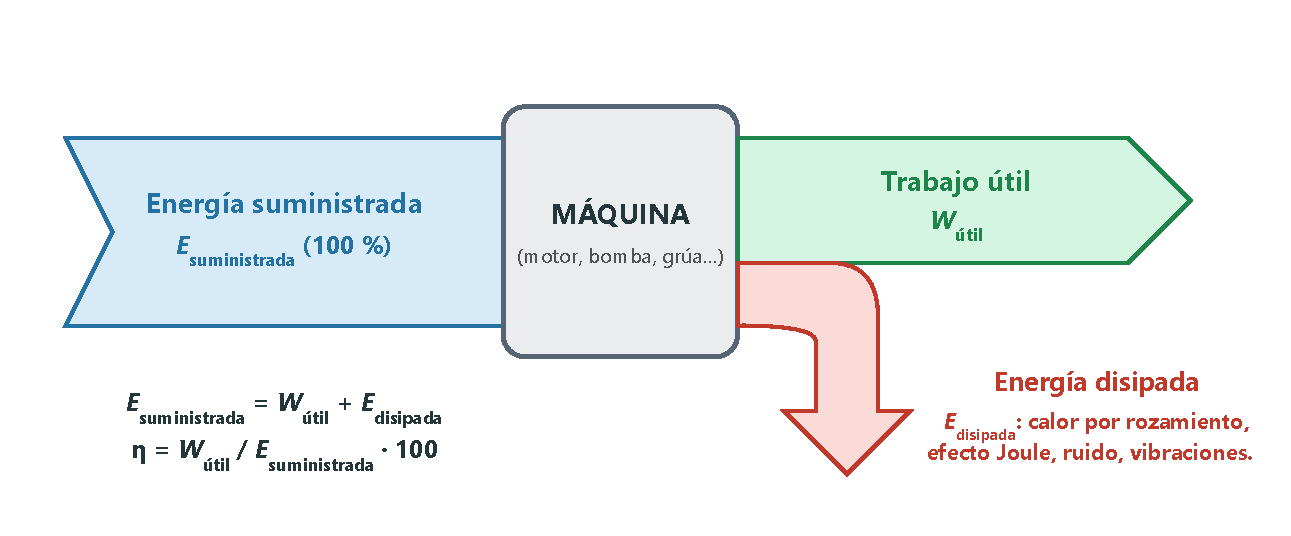
\includegraphics[width=0.8\textwidth]{images/UD12/rendimiento}
    \caption{Balance de energía de una máquina.}
    \label{fig:ud12-rendimiento}
\end{figure}

\begin{definition}[Rendimiento]
    El rendimiento \(\eta\) de una máquina es el cociente, en tanto por ciento, entre el trabajo útil que proporciona y la energía que
    se le suministra (o entre la potencia útil y la potencia consumida):
    \[ \eta = \frac{W_{\text{útil}}}{E_{\text{suministrada}}} \cdot 100 = \frac{P_{\text{útil}}}{P_{\text{consumida}}} \cdot 100 \]
\end{definition}

\begin{itemize}
    \item Siempre es menor que el \qty{100}{\percent}. Lord Kelvin y Max Planck establecieron que es imposible construir una máquina
    térmica que convierta íntegramente en trabajo el calor que recibe (segundo principio de la termodinámica).
    \item Si varias máquinas trabajan en serie, el rendimiento total es el \textbf{producto} de los rendimientos.
    \item Los lubricantes, que reducen el rozamiento, aumentan el rendimiento.
\end{itemize}

\begin{remark}
    \textbf{Rendimiento y eficiencia} no son exactamente lo mismo. La eficiencia es la capacidad de lograr un objetivo con el menor
    consumo de recursos. Una estufa eléctrica tiene un rendimiento cercano al \qty{100}{\percent} (toda la energía eléctrica se
    convierte en calor), pero no sería nada eficiente usarla para enfriar una habitación.
\end{remark}

\begin{example}
    \textbf{Llenar una balsa de riego.} Para regar un olivar se llena una balsa de \qty{500}{\m\cubed} con agua de un pozo de
    \qty{20}{\m} de profundidad. ¿Qué energía hay que suministrar a la bomba si su rendimiento es del \qty{65}{\percent}?
    (\(d_{\text{agua}} = \qty{1000}{\kg\per\m\cubed}\)).

    \textbf{Solución.} El trabajo útil es el aumento de energía potencial del agua:
    \(W_{\text{útil}} = m\,g\,h = 500 \cdot 1000 \cdot \num{9.8} \cdot 20 = \qty{9.8e7}{\joule}\).
    \[ E_{\text{suministrada}} = \frac{W_{\text{útil}}}{\eta} \cdot 100 = \frac{\num{9.8e7}}{65} \cdot 100 = \qty{1.51e8}{\joule} \]
\end{example}

\begin{exercise}
    El motor y los engranajes de la grúa de una obra tienen un rendimiento del \qty{55}{\percent}. ¿Qué energía hay que suministrar
    al motor para subir unas vigas de \qty{800}{\kg} a \qty{20}{\m} de altura?
    \begin{solu}
        \(W_{\text{útil}} = \qty{1.57e5}{\joule}\); \(E = \dfrac{\num{1.57e5}}{\num{0.55}} = \textcolor{red}{\qty{2.85e5}{\joule}}\).
    \end{solu}
\end{exercise}

%========================================================================================
\section{Física en la vida: ITER, un sol en la Tierra}\label{sec:ud12-iter}
%========================================================================================

La humanidad necesita cada vez más energía para mantener su calidad de vida, y las fuentes tradicionales son limitadas o contaminan.
Por eso, científicos de todo el mundo intentan reproducir en la Tierra lo que ocurre en el interior de las estrellas: la \textbf{fusión
nuclear}.

No hay que confundirla con la \textbf{fisión}. En la fisión, un núcleo pesado (normalmente de uranio-235) se rompe en otros más ligeros
al chocar con un neutrón; se liberan energía y nuevos neutrones, que pueden provocar una \textbf{reacción en cadena}. Es lo que ocurre en
las centrales nucleares actuales, que generan residuos radiactivos de larga duración. En la fusión, en cambio, núcleos ligeros (isótopos
del hidrógeno, deuterio y tritio) se unen para formar uno más pesado (helio), como en el Sol. Para que los núcleos, con carga positiva,
venzan su repulsión eléctrica, hay que calentarlos a más de 150 millones de grados.

En una central, la energía nuclear se transforma en energía térmica, que evapora agua; la energía cinética del vapor mueve las
turbinas, y un generador transforma la energía mecánica en eléctrica. La energía se conserva en cada paso, aunque una parte se degrada.

El proyecto internacional \textbf{ITER} (\textit{International Thermonuclear Experimental Reactor}), que se construye en Cadarache
(Francia) con la participación de más de 30 países, pretende demostrar que la fusión es viable. Usa un \textbf{tokamak}, una cámara de
vacío con forma de rosquilla (toroidal) en la que unos potentes imanes mantienen confinado el plasma caliente sin que toque las paredes.
Si se superan los retos técnicos, la fusión sería una fuente casi inagotable de energía, sin emisiones de \ch{CO2} y con muy pocos
residuos: se estima que un gramo de combustible de fusión daría tanta energía como ocho toneladas de petróleo.

\begin{exercise}
    a) Explica la diferencia entre fisión y fusión nuclear. b) El poder calorífico del petróleo es de unos \qty{4.2e7}{\joule\per\kg}.
    ¿Qué energía liberan ocho toneladas de petróleo? ¿Para cuántos hogares bastaría durante un año, si cada uno consume
    \qty{3500}{\kilo\watt\hour} al año? c) Investigad en qué se diferencia el \textit{stellarator}, otro tipo de reactor de fusión, del
    tokamak de ITER.
    \begin{solu}
        a) \textcolor{red}{Fisión}: un núcleo pesado se rompe en otros más ligeros; \textcolor{red}{fusión}: núcleos ligeros se unen
        para formar uno más pesado. b) \(E = 8000 \cdot \num{4.2e7} = \textcolor{red}{\qty{3.4e11}{\joule}} = \qty{9.3e4}{\kilo\watt\hour}\),
        suficiente para unos \textcolor{red}{27 hogares}. c) \textcolor{red}{Respuesta abierta} (el \textit{stellarator} confina el
        plasma solo con imanes de forma retorcida, sin hacer circular corriente por él).
    \end{solu}
\end{exercise}

%========================================================================================
\section{Prácticas}\label{sec:ud12-practicas}
%========================================================================================

\subsection{De energía elástica a energía cinética: un carrete de vasos}

\noindent\begin{minipage}[t]{0.48\textwidth}
    \textbf{Objetivo}
    \begin{itemize}
        \item Comprobar cómo la energía potencial elástica de una goma retorcida se transforma en energía cinética.
    \end{itemize}
\end{minipage}\hfill
\begin{minipage}[t]{0.48\textwidth}
    \textbf{Material}
    \begin{itemize}
        \item Dos vasos de plástico, una pajita, cinta aislante, cuatro gomas elásticas, un clip, un punzón, dos arandelas, tijeras y
        una cinta métrica.
    \end{itemize}
\end{minipage}

\begin{figure}[H]
    \centering
    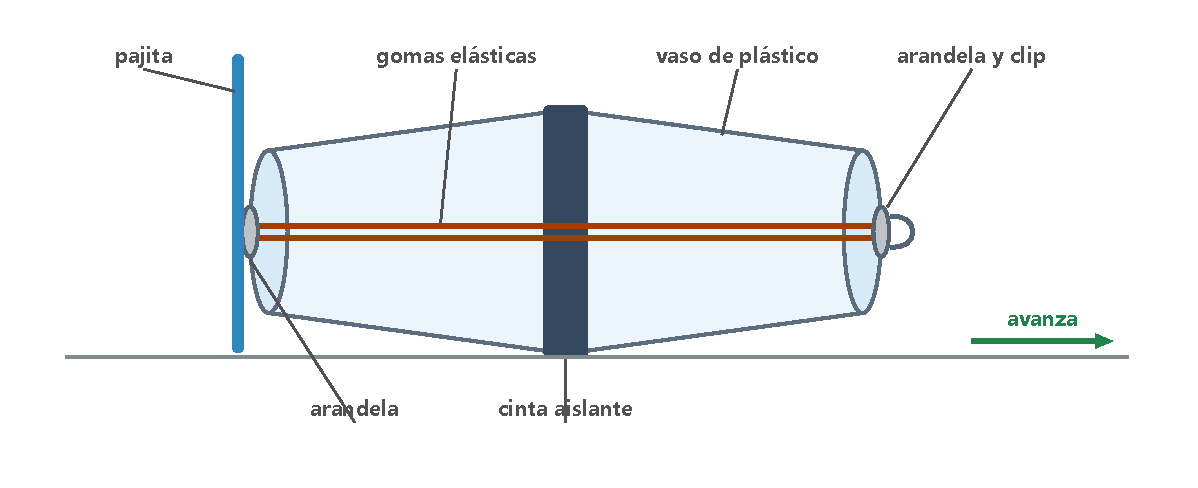
\includegraphics[width=0.75\textwidth]{images/UD12/practica_carrete}
    \caption{Carrete de vasos: al soltarlo, la goma se desenrolla y el carrete avanza.}
    \label{fig:ud12-carrete}
\end{figure}

\textbf{Procedimiento}
\begin{enumerate}[label=\numberballgreen]
    \item Con cuidado, haz un pequeño agujero con el punzón en el centro del fondo de cada vaso.
    \item Une dos gomas para formar una más larga y pásala por el interior de los vasos, sacando un extremo por cada agujero. En un
    extremo, pasa la goma por una arandela y sujétala con el clip; en el otro, pásala por la otra arandela y engánchala a la pajita.
    \item Une las bocas de los vasos con dos vueltas de cinta aislante. La goma debe quedar algo tensa.
    \item Gira la pajita un número de vueltas (10, 20, 30\dots) para retorcer la goma. Apoya el carrete en el suelo sin soltar la
    pajita, suéltala y mide la distancia que recorre. Repite cada medida tres veces.
\end{enumerate}

\begin{exercise}
    a) Describe las transformaciones de energía que se producen desde que giras la pajita hasta que el carrete se para. b) Un grupo
    obtiene estas distancias medias: 10 vueltas, \qty{0.8}{\m}; 20 vueltas, \qty{1.7}{\m}; 30 vueltas, \qty{2.4}{\m}. ¿Qué relación
    observas? c) ¿Por qué acaba parándose el carrete? ¿Se ha perdido la energía?
    \begin{solu}
        a) \textcolor{red}{Química} (de los músculos) \(\rightarrow\) \textcolor{red}{potencial elástica} de la goma \(\rightarrow\)
        \textcolor{red}{cinética} del carrete \(\rightarrow\) \textcolor{red}{térmica} por el rozamiento. b) La distancia es
        \textcolor{red}{aproximadamente proporcional} al número de vueltas: cuanto más se retuerce la goma, más energía almacena.
        c) \textcolor{red}{Por el rozamiento}; la energía no se pierde, se transforma en energía térmica (se degrada).
    \end{solu}
\end{exercise}

\subsection{¿Cuál es nuestra potencia?}

\noindent\begin{minipage}[t]{0.48\textwidth}
    \textbf{Objetivo}
    \begin{itemize}
        \item Calcular la potencia que desarrollamos al subir unas escaleras andando y corriendo.
    \end{itemize}
\end{minipage}\hfill
\begin{minipage}[t]{0.48\textwidth}
    \textbf{Material}
    \begin{itemize}
        \item Un tramo de escaleras, una cinta métrica, un cronómetro (o el móvil) y una báscula.
    \end{itemize}
\end{minipage}

\textbf{Procedimiento}
\begin{enumerate}[label=\numberballgreen]
    \item Mide la altura de un escalón y cuenta los escalones del tramo para calcular la altura total \(h\). Anota tu masa \(m\).
    \item Un compañero cronometra el tiempo que tardas en subir el tramo andando. Repite la medida subiendo deprisa (¡con cuidado!).
    \item Calcula el trabajo que haces contra el peso, \(W = m\,g\,h\), y la potencia, \(P = W/t\), en vatios y en caballos de vapor.
\end{enumerate}

\begin{exercise}
    Una alumna de \qty{60}{\kg} sube 20 escalones de \qty{17}{\cm} en \qty{8.5}{\s} andando y en \qty{3.2}{\s} corriendo. a) Calcula el
    trabajo y la potencia en cada caso. b) ¿Por qué el trabajo es el mismo? c) ¿Es mayor el trabajo realmente hecho por sus músculos?
    \begin{solu}
        a) \(h = \qty{3.4}{\m}\); \(W = \textcolor{red}{\qty{2.0e3}{\joule}}\) en los dos casos; andando, \(P = \textcolor{red}{\qty{235}{\watt}}\);
        corriendo, \(P = \textcolor{red}{\qty{625}{\watt}}\) (\num{0.85}~CV). b) \textcolor{red}{Solo depende de la masa y de la
        altura}, no del tiempo. c) \textcolor{red}{Sí}: el rendimiento de los músculos es bajo (en torno al \qty{25}{\percent}) y gran
        parte de la energía química se transforma en calor.
    \end{solu}
\end{exercise}

%========================================================================================
\section{Situación de aprendizaje: guardar la energía del sol y del viento (ODS 7)}\label{sec:ud12-ods}
%========================================================================================

El \textbf{ODS 7} pide garantizar el acceso a una energía asequible, segura, sostenible y moderna para todos. Desde 2010, más de mil
millones de personas han conseguido electricidad, pero cientos de millones todavía viven sin ella. Al mismo tiempo, para frenar el
cambio climático hay que \textbf{descarbonizar}: sustituir el carbón, el petróleo y el gas por energías renovables. España tiene un
gran potencial solar y eólico, y empresas españolas han sido líderes mundiales en este sector.

Pero el sol y el viento no siempre están disponibles cuando hace falta la energía. Una solución son las \textbf{centrales hidroeléctricas
de bombeo}: cuando sobra electricidad (por ejemplo, a mediodía, con mucha producción solar), se usa para bombear agua desde un embalse
inferior a otro superior; cuando falta, se deja caer el agua y se genera electricidad. Funcionan como una enorme «batería» de energía
potencial gravitatoria. Muy cerca de Almansa, en Cortes de Pallás (Valencia), está el complejo de La Muela, uno de los mayores de Europa,
con un desnivel de unos \qty{500}{\m} entre sus depósitos.

\begin{marker}
    \textbf{Reto:} por grupos, preparad un informe sobre cómo almacenar la energía renovable para que llegue a todos a cualquier hora.
\end{marker}

\begin{enumerate}[label=\numberballred]
    \item \textbf{Investigad} distintas formas de almacenar energía: centrales de bombeo, baterías, hidrógeno verde, sales fundidas en
    centrales termosolares. ¿Qué transformaciones de energía hay en cada una?
    \item \textbf{Calculad} la energía que almacena una central de bombeo (ejercicio siguiente).
    \item \textbf{Analizad} el impacto ambiental de las renovables, con sus ventajas e inconvenientes frente a las no renovables, y qué
    es una vivienda bioclimática.
    \item \textbf{Comunicad} vuestras propuestas para un consumo de energía más sostenible y responsable en vuestro centro.
\end{enumerate}

\begin{exercise}
    El depósito superior de una central de bombeo almacena \qty{2e7}{\m\cubed} de agua con un desnivel de \qty{500}{\m}. a) ¿Qué
    energía potencial almacena, en julios y en kWh? b) Si el rendimiento del ciclo completo (bombear y turbinar) es del \qty{75}{\percent},
    ¿qué energía eléctrica devuelve? c) ¿A cuántos hogares podría abastecer durante un día, si cada uno consume \qty{3500}{\kilo\watt\hour}
    al año?
    \begin{solu}
        a) \(E_p = \num{2e10} \cdot \num{9.8} \cdot 500 = \textcolor{red}{\qty{9.8e13}{\joule}} = \textcolor{red}{\qty{2.7e7}{\kilo\watt\hour}}\)
        (27~GWh). b) \(\textcolor{red}{\qty{2.0e7}{\kilo\watt\hour}}\). c) Cada hogar consume \qty{9.6}{\kilo\watt\hour} al día:
        unos \textcolor{red}{2,1 millones de hogares}.
    \end{solu}
\end{exercise}
